\documentclass[a0,portrait]{a0poster}
\usepackage{abll-poster}
\usepackage{multicol}
\usepackage{graphicx}
\usepackage{wrapfig}
\setlength{\columnsep}{60pt}

\newcommand{\Ca}{C$_{\alpha}${}}


\begin{document}
\ULCornerWallPaper{1.0}{ku-background.pdf}
\fontsize{40pt}{60pt}\selectfont

\begin{textblock}{100}(0,0)
\Faculty{\an{department of computer science}}
\\
\Department{\an{university of copenhagen}}
\end{textblock}

\begin{textblock}{100}(0,7)
\Title{Fitting an All-atom Protein Model to a $C_\alpha$-trace}
\end{textblock}

\begin{textblock}{100}(0,13.5)
\Authors{Martin Dybdal, Anders Boesen Lindbo Larsen and Esben Skaarup}
\\[-8mm]
\AuthorEmails{\texttt{dybber@dybber.dk}, \texttt{abll@diku.dk} and \texttt{sben@diku.dk}}
\end{textblock}

\linespread{1.075}\fontsize{28pt}{40pt}\selectfont

\begin{GridBlock}{0}{21}{100}
\begin{multicols}{3}
\Head{Summary}
%Protein structure prediction can be simplified by using a model that only includes a subset of the atoms present in proteins. In particular, the algorithms group at our department only predicts a folding of the \Ca-trace, and are thus excluding most backbone atoms and all side-chain molecules.

In this work we investigate a strategy for predicting the structure of proteins. Given a so-called \emph{\Ca-trace}, we wish to fold the protein to match the trace.

%The strategy divides the problem into two separate tasks.


\section{Motivation}
\begin{itemize}
    \item[-- ] Proteins are the perhaps most important molecules of
      living organisms.
    \item[-- ] Computational resolution of the protein 3D-structure has
      many applications in biotechnology and medicine.
    \item[-- ] Protein structure prediction and the related topic protein
      folding, are large and active research fields.
    \end{itemize}

\section{Our problem}
Currently, we are only able to predict protein structures at the $C_\alpha$-trace level. 
Our goal with this project is
to extend this model with the remaining atoms to get an all-atom
model.  This will also enable the algorithms group to participate in
the CASP experiment \cite{caspwebsite}.

The strategy we will pursue, is to use a given $C_\alpha$-trace as target when fitting a
protein model that contains all atoms. The fitting should be conducted,
such that it minimizes the number of clashes and at the same time
minimizes the deviation from the target $C_\alpha$-trace.

We consider our fitting problem as two somewhat separate problems.
First, the backbone must be fitted to the \Ca-trace by minimizing
the deviation from the $C_{\alpha}$-trace.  Hereafter, the amino acid
side-chains are added to the backbone.  In the following we have chosen to
consider these two tasks separately.
%However, as we shall see in Section \ref{sec:evaluation_handling_side-chains}, the performance of our residue handling depends heavily on the backbone fitting.
 % (even though the residue handling might require us to adjust the backbone).

In Section \ref{chap:fitting_backbone}, we will describe the strategy we use to fit the all-atom backbone to the \Ca-trace ignoring the amino acid residues.
In Section \ref{chap:handling_sidechains}, we will explain how we add the side-chains to the all-atom backbone changing the backbone-conformation only if necessary.

\begin{wrapfigure}{r}{.3\columnwidth}
\vspace{-.8cm}
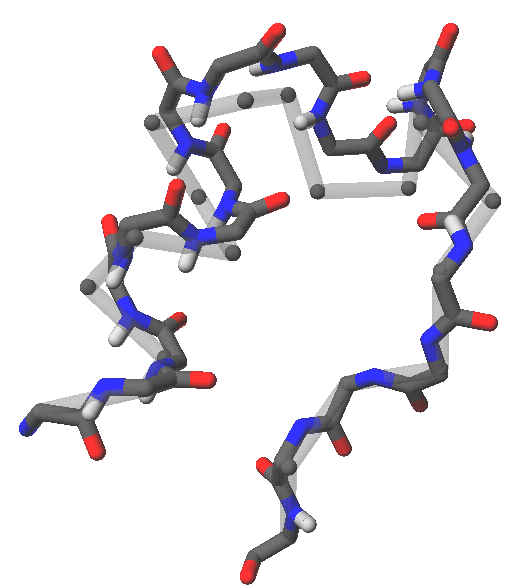
\includegraphics[width=.3\columnwidth]{../rapport/figures/forside.png}
\vspace{-3.5cm}
\end{wrapfigure}

\end{multicols}
\end{GridBlock}

\begin{GridBlock}{0}{45}{100}
\begin{wraptable}{r}{0.75\textwidth}
\addtolength\leftskip{9mm}
  \begin{tabular}{lrr}
    \toprule
    \multicolumn{1}{c}{Bond} & \multicolumn{1}{c}{Avg. length} & \multicolumn{1}{c}{Std.dev.} \\ \midrule
    C-O   & 1.2260 Å & 0.0188 Å\\
    CA-C  & 1.5272 Å & 0.0191 Å\\
    N-CA  & 1.4680 Å & 0.0237 Å\\
    C-N   & 1.3234 Å & 0.0215 Å\\
    N-H   & 0.9793 Å & 0.0342 Å\\
    CA-CB & 1.5327 Å & 0.0228 Å\\
    CA-HA & 1.0747 Å & 0.0307 Å\\ \bottomrule
  \end{tabular}
  \label{tab:average_bond_lengths}
  \caption{Average bond lengths (in ångstrøm)}
\end{wraptable}
  \Head{Protein structure} 
  \textit{Bond lengths} are the distances between the covalently bonded atoms
in a molecule (usually measured in ångstrøm). We will name the
individual bond lengths by the name of the two atoms which the bond
connects. For example, the bond between a \Ca\ and N atom in an amino acid of
the protein backbone is called \Ca -N. We have computed bond lengths
for all bonds in the backbone, the results are shown in Table
\ref{tab:average_bond_lengths}. As can be seen from the last column in
the table, the variation is very limited and we therefore have not
found it necessary to consider any variations from the mean
lengths.
\end{GridBlock}

\begin{GridBlock}{0}{40}{100}
%\begin{wrapfigure}{r}{0.5\textwidth}
 \begin{center}
\resizebox{10\TPHorizModule}{!}{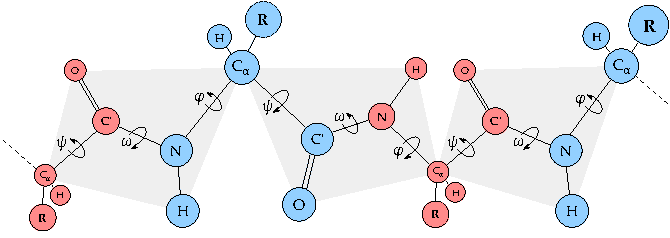
\includegraphics{../rapport/figures/protein-torsion-angles.pdf}}
\textbf{Figure 1}: Protein torsion angles
 \end{center}
%\end{wrapfigure}
\end{GridBlock}

\begin{GridBlock}{0}{55}{48}
\Head{Backbone fitting}
\textit{Bond lengths} are the distances between the covalently bonded atoms
in a molecule (usually measured in ångstrøm). We will name the
individual bond lengths by the name of the two atoms which the bond
connects. For example, the bond between a \Ca\ and N atom in an amino acid of
the protein backbone is called \Ca -N. We have computed bond lengths
for all bonds in the backbone, the results are shown in Table
\ref{tab:average_bond_lengths}. As can be seen from the last column in
the table, the variation is very limited and we therefore have not
found it necessary to consider any variations from the mean
lengths.
\end{GridBlock}

\begin{GridBlock}{51}{55}{48}
\begin{wrapfigure}{r}{0.55\textwidth}
    \centering
    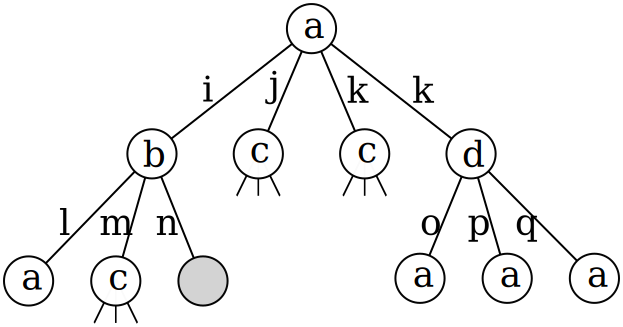
\includegraphics[width=.45\textwidth]{../rapport/figures/rotamersearch}
    \caption{The structure of our rotamer search space when
      eliminating collisions with the amino acid \textit{a}.}
    \label{fig:rotamer-search-tree}
\end{wrapfigure}
\Head{Rotamer selection}
\textit{Bond lengths} are the distances between the covalently bonded atoms
in a molecule (usually measured in ångstrøm). We will name the
individual bond lengths by the name of the two atoms which the bond
connects. For example, the bond between a \Ca\ and N atom in an amino acid of
the protein backbone is called \Ca -N. We have computed bond lengths
for all bonds in the backbone, the results are shown in Table
\end{GridBlock}

%\begin{GridBlock}{51}{80}{48}
%\Head{Conclusion}
%\begin{itemize}
%\item[-- ] We can obtain a RMSD of less than $0.2$ Å with our devised
%  variant of cyclic coordinate descent
%\item[-- ] Selecting the appropriate rotamers makes it possible to
%  reduce the number collisions to 1 for every 4700 amino acids on a
%  realistic protein.
%\end{itemize}
%\end{GridBlock}


% If you want to add a figure do something like this:




\end{document}

